\section{Мета роботи}
Закріпити теоретичні знання та набути практичного досвіду
впорядкування набору статичних та динамічних структур даних.

\noindent
\textbf{Теми для попередньої роботи:}
\begin{itemize}
    \item масиви та списки;
    \item класифікація алгоритмів сортування;
    \item алгоритми сортування вибором (вибіркою) та включенням.
\end{itemize}


\section{Завдання}
Написати програму, що реалізує сортування статичного та/або
динамічного набору даних заданим способом згідно з даними табл. 11.1.

Визначити кількість порівнянь та обмінів для наборів даних, що
містять різну кількість елементів (20, 1000, 5000, 10000, 50000).

Оцінити час сортування. Дослідити вплив початкової впорядкованості
набору даних (відсортований, відсортований у зворотному порядку,
випадковий).


\section{Хід виконання}
Для виконання завдання було обрано мову Rust.
Увесь код також додатково був розміщений в GitHub репозитарії: \href{https://github.com/blackgolyb/algos-labs}{https://github.com/blackgolyb/algos-labs}.


\newpage
\subsection{Підготовка до виконання}
Для подальшої роботи підготуємо набір функцій, інтерфейсів та макросів.

\subsubsection{Logger}
Створимо структуру Logger та Metrics.
Logger буде відповідати за логування сортування та по закінченню роботи буде видавати Metrics.
Metrics в свою чергу буде зберігати в собі результати логування сортування.
\lstinputlisting[language=Rust, style=colouredRust]{\codeDirectory/src/libs/sort/logger.rs}

\subsubsection{Інтерфейси}
Також створимо інтерфейси які повинен буде реалізувати наше сортування: Sort, SortLogging.
\lstinputlisting[language=Rust, style=colouredRust]{\codeDirectory/src/libs/sort/traits.rs}

\subsubsection{Макроси}
Для зручного створення сортування напишемо пару макросів які будуть додавати зручний DSL.
Так як більшість сортування можна описати функцією яка приймає масив по змінювальному посиланню та сортує всередені цього масива.
То ми можемо звести створення сортуваня до створення однієї функції яка буде його реалізовувати,
а створення структури та додавання логування покласти на наш DSL.
\lstinputlisting[language=Rust, style=colouredRust]{\codeDirectory/src/libs/sort/macros.rs}

\subsubsection{Тестування}
Також додамо декілька функцій для того щоб тестувати наші сортування та зберігати результати їх логування.
\lstinputlisting[language=Rust, style=colouredRust]{\codeDirectory/src/libs/sort/testing.rs}


\newpage
\subsection{Сортування}
\lstinputlisting[language=Rust, style=colouredRust]{\codeDirectory/src/libs/sort/variants/bubble.rs}


\newpage
\subsection{Приклад роботи програми}
\noindent
Код програми для перевірки:
\lstinputlisting[language=Rust, style=colouredRust]{\codeDirectory/src/labs/lab11/main.rs}


\begin{figure}[ht!]
    \centering
    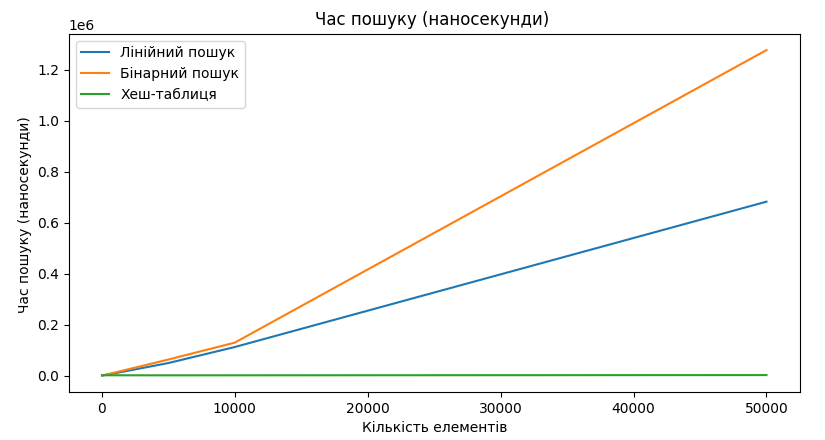
\includegraphics[width=.8\textwidth]{\assetsDirectory/time.png}
    \caption{Залежність часу пошуку від кількості елементів}
\end{figure}
\begin{figure}[ht!]
    \centering
    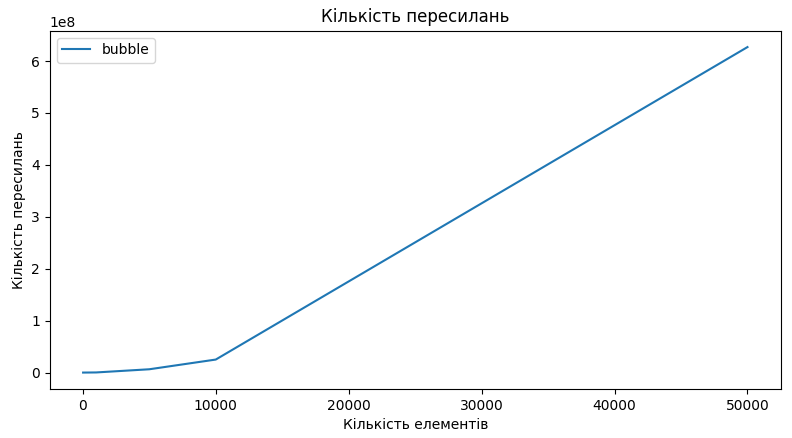
\includegraphics[width=.8\textwidth]{\assetsDirectory/swap.png}
    \caption{Залежність кількості пересилань від кількості елементів}
\end{figure}
\begin{figure}[ht!]
    \centering
    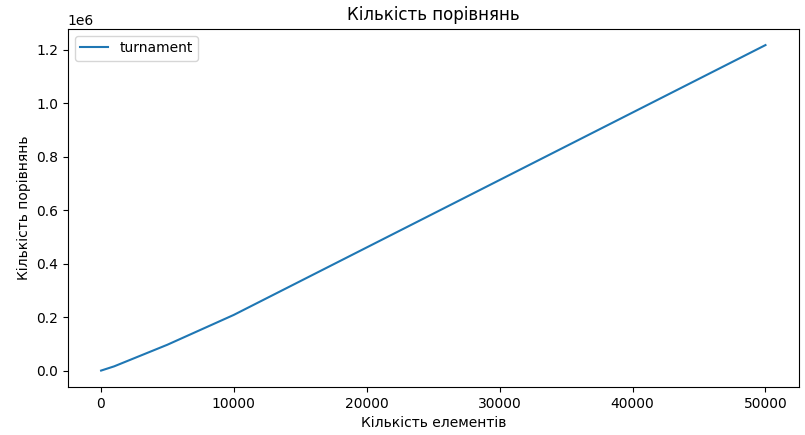
\includegraphics[width=.8\textwidth]{\assetsDirectory/comp.png}
    \caption{Залежність кількості порівнянь від кількості елементів}
\end{figure}


\newpage
\section{Висновки}
В ході виконання лабораторної робити було створено сортування bubble sort.
Також було протестовано його на різних обємах даних та побудовано графіки для наглядної демонстрації його характеристик.
